\documentclass[final,hyperref={pdfpagelabels=false}]{beamer}
\usepackage{grffile}
\mode<presentation>{\usetheme{byu}}
\usepackage[english]{babel}
\usepackage[latin1]{inputenc}
\usepackage{amsmath,amsthm, amssymb, latexsym}
\usepackage{wrapfig}
\boldmath
\usepackage[orientation=landscape,size=a0,scale=1.5]{beamerposter}
\usepackage{array,booktabs,tabularx}
\newcolumntype{Z}{>{\centering\arraybackslash}X} \listfiles
\graphicspath{{figures/}}
\title{\huge Firefly Assembler: Parallelizing the Assembly of Genome Fragments}
\author{Kyle Corbitt, Dan Haskin}
\institute[Brigham Young University]{Molecular Biology and Computer Science Departments}
\date[Nov. 20th, 2013]{Nov. 20th, 2013}
\newlength{\columnheight}
\setlength{\columnheight}{105cm}
\begin{document}
\begin{frame}
    \begin{columns}
        \begin{column}{.32\textwidth}
            \begin{beamercolorbox}[center,wd=\textwidth]{postercolumn}
                \begin{minipage}[T]{.95\textwidth}
                    \parbox[t][\columnheight]{\textwidth}{
                        \begin{block}{Purpose}
                            Our purpose is to create a genome assembler based
                            on a novel approach called the Firefly Algorithm
                            (1).  We hypothesize that this will produce more
                            accurate assemblies than other assemblers.
                        \end{block}
                        \begin{block}{Introduction}
                            Currently the computational time required to
                            accurately assemble a de novo genome is a
                            significant bottleneck in bioinformatics.
                            Algorithms exist that can assemble a genome in a
                            relatively short time, but these algorithms
                            typically are not able to guarantee an accurate
                            assembly. Conversely, algorithms exist that can
                            guarantee an accurate assembly of reads but that
                            are unacceptably inefficient.  By modeling genome
                            assembly as a Travelling Salesman Problem (TSP), we
                            show how established algorithms for getting
                            near-optimal results on that problem can be used
                            for the purpose of solving the genome assembly
                            problem.
                        \end{block}
                        \begin{block}{Graph Representation}
                            In order to apply the LocalSearch and Firefly
                            algorithms to an assembly task we must first
                            represent the assembly as a graph.  An intuitive
                            method of accomplishing this is shown below.
                            \begin{center}
                                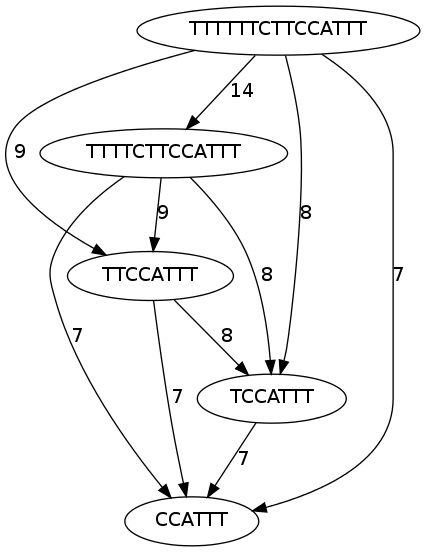
\includegraphics[scale=0.75]{example_graph}
                            \end{center}
                            Each node in the graph represents a short read. The
                            edges connecting the nodes represent overlaps.  The
                            challenge of assembly then becomes finding a path
                            through the graph that connects all the nodes,
                            using a route that is as "long" as possible
                            (contains the greatest possible number of overlaps).
                       \end{block}
                } \end{minipage}
            \end{beamercolorbox}
        \end{column}
        \begin{column}{.32\textwidth}
            \begin{beamercolorbox}[center,wd=\textwidth]{postercolumn}
                \begin{minipage}[T]{.95\textwidth}
                    \parbox[t][\columnheight]{\textwidth}{
                        \begin{block}{Greedy Algorithm}
                            As a base line, we use the greedy algorithm to
                            traverse the sequence overlap graph.  In essence,
                            the greatest overlaps are added to the path through
                            the graph first, followed by subsequent overlaps
                            added later to complete the path through the graph,
                            in order from greatest overlap to least.  This
                            algorithm is similar or equivalent to the
                            conventional shotgun sequencing technique used in
                            many sequence assemblers today.
                        \end{block}
                        \begin{block}{LocalSearch Algorithm}
                            The LocalSearch algorithm works by taking an
                            initial sequencing and then trying different small
                            variations on it to find a "better" graph traversal
                            (a longer traversal through the overlap graph).
                        \end{block}
                        \begin{block}{Firefly Algorithm}
                            In the firefly algorithm, A number of
                            random paths through the graph are generated, and
                            each one is called a "firefly". The algorithm
                            starts "moving" the fireflies (changing the paths)
                            toward other fireflies based on how "bright" (good)
                            they are, and how "close" (similar) they are to
                            each other, as shown below.
                            \begin{center}
                                \includegraphics[scale=1.5]{example_firefly}
                            \end{center}
                            {\em {\small photo courtesy of \url{http://www.mathworks.com/matlabcentral/fx_files/38931/3/SwarmFireFly_distance.jpg}. } }
                             
                        \end{block}
                    }
        \end{minipage}
    \end{beamercolorbox}
        \end{column}
        \begin{column}{.32\textwidth}
            \begin{beamercolorbox}[center,wd=\textwidth]{postercolumn}
                \begin{minipage}[T]{.95\textwidth}
                    \parbox[t][\columnheight]{\textwidth}{
                        \begin{block}{Introduction}
                            Something way cool here.
                        \end{block}
                        \begin{block}{Introduction}
                            Something way cool here.
                        \end{block}
                        \begin{block}{Introduction}
                            Something way cool here.
                        \end{block}
                        \begin{block}{Introduction}
                            Something way cool here.
                        \end{block}
                        \begin{block}{Introduction}
                            Something way cool here.
                        \end{block}
                    }
                \end{minipage}
            \end{beamercolorbox}
        \end{column}
    \end{columns}
    \vskip1ex
    \tiny\hfill{Created with \LaTeX \texttt{beamerposter}  \url{http://www-i6.informatik.rwth-aachen.de/~dreuw/latexbeamerposter.php} \hskip1em}
\end{frame}
\end{document}
